\documentclass[12pt,letterpaper]{article}

\usepackage[margin=0.85in]{geometry}
\usepackage[T1]{fontenc}
\usepackage{lmodern}
\usepackage[scaled=0.95]{helvet}
\renewcommand{\familydefault}{\sfdefault}
\usepackage{amsmath}
\usepackage{array}
\usepackage{tabularx}
\usepackage[table]{xcolor}
\usepackage{tikz}
\usetikzlibrary{arrows.meta,shapes.geometric}
\usepackage[most]{tcolorbox}
\usepackage{titlesec}
\usepackage{fancyhdr}
\usepackage{needspace}

% ---------- Colors ----------
\definecolor{robo}{HTML}{1F6FB5}      % Cookie Monster blue
\definecolor{robodark}{HTML}{7A4A22}  % cookie brown
\definecolor{elmo}{HTML}{D32F2F}
\definecolor{oscar}{HTML}{4C8C2B}
\definecolor{cookie}{HTML}{C68B4E}
\definecolor{chip}{HTML}{3B2314}
\definecolor{itc}{HTML}{6B3FA0}     % The Count purple
\definecolor{flip}{HTML}{C0392B}
\definecolor{softyellow}{HTML}{FFF6DD}
\definecolor{softblue}{HTML}{E8F1FA}
\definecolor{softpurple}{HTML}{F1EBF8}
\definecolor{softgray}{HTML}{F3F3F3}
\definecolor{gold}{HTML}{C68B4E}

% ---------- Headings ----------
\titleformat{\section}{\Large\bfseries\color{robodark}}{}{0pt}{}
\titlespacing*{\section}{0pt}{14pt}{6pt}
\setcounter{secnumdepth}{0}

\pagestyle{fancy}
\fancyhf{}
\renewcommand{\headrulewidth}{0pt}
\fancyfoot[C]{\small\color{gray}The Cookie Circle \textperiodcentered\ page \thepage}

\setlength{\parindent}{0pt}
\setlength{\parskip}{6pt}

% ---------- Helpers ----------
% A cookie with chocolate chips
\newcommand{\cookie}[1][1]{%
  \begin{tikzpicture}[scale=#1, baseline=-0.6ex]
    \fill[cookie] (0,0) circle (0.5);
    \draw[robodark, line width=0.8pt] (0,0) circle (0.5);
    \foreach \x/\y in {-0.2/0.2, 0.15/0.25, 0.25/-0.1, -0.1/-0.25, -0.28/-0.05, 0.05/0.0}
      \fill[chip] (\x,\y) circle (0.06);
  \end{tikzpicture}}

\newcommand{\blank}[1][3cm]{\underline{\hspace{#1}}}

\newcounter{question}
\newcommand{\question}{%
  \refstepcounter{question}\par\needspace{3\baselineskip}%
  \textbf{\color{robo}Question \arabic{question}.}~}

\newtcolorbox{bigidea}[1][]{enhanced, colback=softyellow, colframe=gold,
  boxrule=1pt, arc=3mm, left=8pt, right=8pt, top=6pt, bottom=6pt, #1}
\newtcolorbox{tryit}{enhanced, colback=softblue, colframe=robo,
  boxrule=0.8pt, arc=3mm, left=8pt, right=8pt}
\newtcolorbox{mathclub}[1]{enhanced, colback=softpurple, colframe=itc,
  boxrule=0.8pt, arc=3mm, left=8pt, right=8pt, top=4pt, bottom=4pt,
  title={\textbf{#1}}, colbacktitle=itc, coltitle=white}

\renewcommand{\arraystretch}{1.6}

\begin{document}

% ================= Title =================
\begin{center}
  {\cookie[0.9]\hspace{0.6em}\cookie[0.9]\hspace{0.6em}\cookie[0.9]}\\[6pt]
  {\Huge\bfseries\color{robodark} The Cookie Circle}\\[4pt]
  {\Large Imaginary Numbers and Euler's Equation}\\[6pt]
  {\small\color{gray} November 4, 2026 \textperiodcentered\ Nathaniel}
\end{center}

\vspace{2pt}
Name: \blank[6cm] \hfill Date: \blank[4cm]

% ================= The story =================
\section{The story}

\textbf{\color{elmo}Elmo} loves to dance on the number line! Elmo stands on a number and faces
the way the numbers grow. Elmo knows two dance moves: \textbf{walking} and \textbf{turning}.

\textbf{\color{robo}Cookie Monster} has baked one GIANT cookie, and \textbf{\color{itc}The Count}
has a very tricky riddle. To solve it, Elmo will discover a whole new kind of number, and one
of the most famous equations in all of math!

% ================= Flip =================
\section{Oscar's opposite trick: times $-1$ means ``turn around''}

\begin{center}
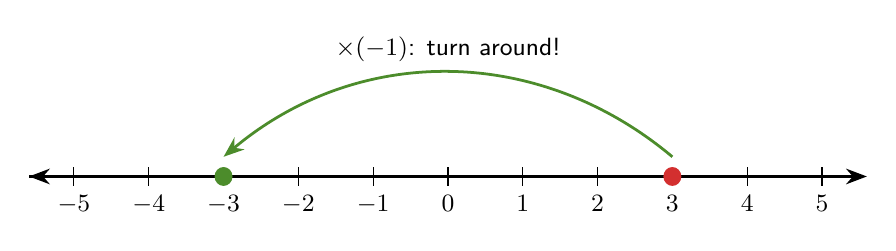
\begin{tikzpicture}[x=0.95cm]
  \draw[-{Stealth}, line width=1pt] (-5.6,0) -- (5.6,0);
  \draw[{Stealth}-, line width=1pt] (-5.6,0) -- (0,0);
  \foreach \n in {-5,...,5} {
    \draw (\n,0.12) -- (\n,-0.12);
    \node[below, font=\small] at (\n,-0.12) {$\n$};
  }
  \fill[elmo] (3,0) circle (0.12);
  \fill[oscar] (-3,0) circle (0.12);
  \draw[-{Stealth}, oscar, line width=1pt] (3,0.25) to[bend right=40]
    node[above, font=\small, black] {$\times(-1)$: turn around!} (-3,0.25);
\end{tikzpicture}
\end{center}

\begin{bigidea}
\textbf{\color{oscar}Oscar the Grouch} loves opposites! His favorite trick is multiplying by
$-1$. It is a \textbf{half turn}: Elmo spins around to face the other way, and the number jumps
to the other side of 0. So $3 \times (-1) = -3$. \emph{``Scram! Go the other way!''}
\end{bigidea}

\question $4 \times (-1) = $ \blank[2cm]

\vspace{4pt}
\question Turn around \emph{two} times: $2 \times (-1) \times (-1) = $ \blank[2cm]\\[4pt]
Which way is Elmo facing now? \blank[3cm]

\begin{tryit}
\textbf{Try it!} Stand up and face the board. Do a half turn. Do another half turn. Which way
are you facing?
\end{tryit}

% ================= Quarter turn =================
\newpage
\section{The tricky riddle}

\textbf{\color{itc}The Count} asks: \emph{``Is there a number that, if you multiply by it
\textbf{two} times, makes Elmo turn around? Ah ah ah!''}

\question Elmo tries. Fill in the blanks.

\begin{center}
\begin{tabular}{l@{\hspace{2em}}l}
$1 \times 1 = $ \blank[1.6cm] & Did Elmo turn around? \blank[2cm] \\
$(-1) \times (-1) = $ \blank[1.6cm] & Did Elmo turn around? \blank[2cm] \\
\end{tabular}
\end{center}

Nothing on the number line works! Elmo needs a brand new idea.

\section{Elmo's quarter turn, $i$}

\begin{tryit}
\textbf{Try it!} Do a half turn using \textbf{two quarter turns}: turn left a little (a quarter
turn), then turn left again. You are facing backwards. It worked!
\end{tryit}

\begin{center}
\begin{tikzpicture}[scale=0.9]
  \draw[-{Stealth}, line width=1pt] (-3.4,0) -- (3.4,0);
  \draw[-{Stealth}, line width=1pt] (3.4,0) -- (-3.4,0);
  \draw[-{Stealth}, line width=1pt, itc] (0,-3.4) -- (0,3.4);
  \draw[-{Stealth}, line width=1pt, itc] (0,3.4) -- (0,-3.4);
  \foreach \n in {-3,...,3} \draw (\n,0.1) -- (\n,-0.1);
  \foreach \n in {-3,...,-1,1,2,3} \draw[itc] (0.1,\n) -- (-0.1,\n);
  \node[below right, font=\small] at (2,0) {$2$};
  \node[below left, font=\small] at (-2,0) {$-2$};
  \node[right, font=\small, itc] at (0.1,2) {$2i$};
  \node[right, font=\small, itc] at (0.1,-2) {$-2i$};
  \fill[elmo] (2,0) circle (0.12);
  \fill[itc] (0,2) circle (0.12);
  \fill[oscar] (-2,0) circle (0.12);
  \draw[-{Stealth}, itc, line width=1pt] (2.15,0.3) to[bend right=35]
    node[above right, font=\small] {$\times i$} (0.3,2.15);
  \draw[-{Stealth}, itc, line width=1pt] (-0.3,2.15) to[bend right=35]
    node[above left, font=\small] {$\times i$} (-2.15,0.3);
  \node[font=\small, align=center] at (4.6,2.5) {\textcolor{itc}{\textbf{new}}\\
    \textcolor{itc}{\textbf{up-down line!}}};
\end{tikzpicture}
\end{center}

\begin{bigidea}
Mathematicians invented a new number called $\boldsymbol{i}$. Multiplying by $i$ is a
\textbf{quarter turn} to the left. It makes Elmo dance off the number line onto a new
\textbf{up-down line}. Numbers on the up-down line are called \textbf{imaginary numbers}.

Two quarter turns make a half turn, so \quad $i \times i = -1$. \quad Riddle solved!
\end{bigidea}

% ================= Turn table =================
\newpage
\section{The turning pattern}

Elmo starts at $1$ and keeps multiplying by $i$. Each time, Elmo does one more quarter turn,
and The Count counts them: \emph{``ONE quarter turn! TWO quarter turns! Ah ah ah!''}
Use the picture on the page before to fill in where Elmo lands.

\begin{center}
\renewcommand{\arraystretch}{1.7}
\rowcolors{2}{white}{softpurple}
\begin{tabular}{|>{\centering\arraybackslash}p{3.6cm}|>{\centering\arraybackslash}p{3.6cm}|>{\centering\arraybackslash}p{3.6cm}|}
\hline
\rowcolor{itc}
\textbf{\color{white}Quarter turns} & \textbf{\color{white}Elmo is at} & \textbf{\color{white}Pointing} \\
\hline
0 & $1$ & right \\ \hline
1 & $i$ & up \\ \hline
2 &     &    \\ \hline
3 &     &    \\ \hline
4 &     &    \\ \hline
\end{tabular}
\end{center}

\question How many quarter turns bring Elmo all the way back to $1$? \blank[2cm]

\vspace{4pt}
\question The pattern repeats! Where is Elmo after 8 quarter turns? (Count by 4s.) \blank[2cm]

% ================= Map =================
\section{Cookie Monster's cookie map}

Now numbers can go \textbf{sideways} and \textbf{up}! Cookie Monster hid cookies all over the
map. A number like $2 + 1i$ is an address: walk $2$ steps right, then $1$ step up.
\emph{``Me want cookie at that address!''}

\begin{center}
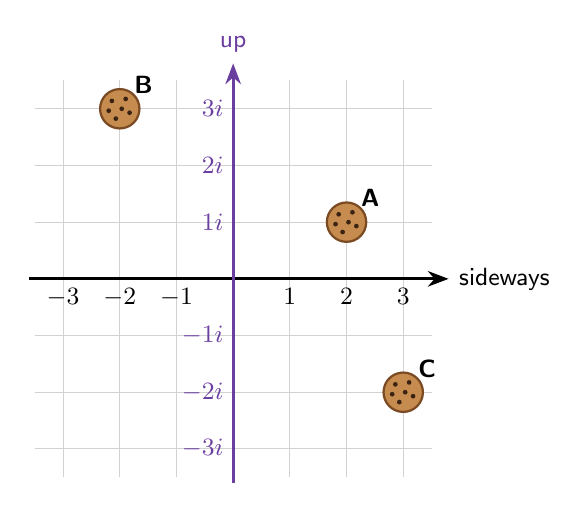
\begin{tikzpicture}[scale=0.72]
  \draw[step=1, gray!35] (-3.5,-3.5) grid (3.5,3.5);
  \draw[-{Stealth}, line width=1pt] (-3.6,0) -- (3.8,0) node[right, font=\small] {sideways};
  \draw[-{Stealth}, line width=1pt, itc] (0,-3.6) -- (0,3.8) node[above, font=\small] {up};
  \foreach \n in {-3,...,-1,1,2,3} {
    \node[below, font=\small] at (\n,0) {$\n$};
    \node[left, font=\small, itc] at (0,\n) {$\n i$};
  }
  % cookies
  \foreach \x/\y/\l in {2/1/A, -2/3/B, 3/-2/C} {
    \node at (\x,\y) {\cookie[0.5]};
    \node[font=\bfseries\small] at (\x+0.42,\y+0.42) {\l};
  }
\end{tikzpicture}
\end{center}

\question Cookie \textbf{A} is at $2 + 1i$. Write the addresses of cookies B and C.

\begin{center}
\textbf{B}: \blank[1.2cm] $+$ \blank[1.2cm]$\,i$
\qquad
\textbf{C}: \blank[1.2cm] $+$ \blank[1.2cm]$\,i$
\end{center}

\question Cookie Monster hid one more cookie at $1 + 3i$. Draw it on the map!

% ================= Circle and Euler =================
\newpage
\section{Elmo walks around the giant cookie}

\begin{tryit}
\textbf{Try it!} Wrap a string once around a cup (or a real cookie!). Then lay the string
flat and count how many cup-widths fit along it, like The Count: \emph{``ONE! TWO! THREE!
And a little bit more! Ah ah ah!''}
\end{tryit}

\question About how many cup-widths long was the string? \blank[2cm]

\begin{bigidea}
It is always a little more than 3, for \emph{every} circle! That number is called
\textbf{pi}, written $\boldsymbol{\pi}$. It is about $3.14$.

If a cookie is 2 steps wide, the edge all the way around is $2\pi$ steps long, so
\textbf{halfway around is exactly $\pi$ steps}.
\end{bigidea}

Elmo starts at $1$ and walks around the edge of Cookie Monster's giant cookie, which is 2 steps
wide. Fill in the boxes with where Elmo lands: $1$, $i$, $-1$, or $-i$.

\begin{center}
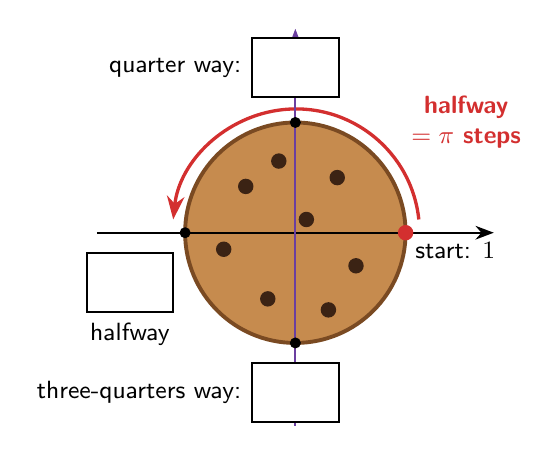
\begin{tikzpicture}[scale=1.4]
  \fill[cookie] (0,0) circle (1);
  \foreach \x/\y in {-0.45/0.42, 0.38/0.5, 0.55/-0.3, -0.25/-0.6, -0.65/-0.15, 0.1/0.12, 0.3/-0.7, -0.15/0.65}
    \fill[chip] (\x,\y) circle (0.07);
  \draw[line width=1.4pt, robodark] (0,0) circle (1);
  \draw[-{Stealth}, line width=1.2pt, elmo] (1.12,0.12) arc (6:174:1.12);
  \node[elmo, font=\small\bfseries, align=center] at (1.55,1.0) {halfway\\$= \pi$ steps};
  \draw[-{Stealth}, line width=0.8pt] (-1.8,0) -- (1.8,0);
  \draw[-{Stealth}, line width=0.8pt, itc] (0,-1.75) -- (0,1.85);
  \fill[elmo] (1,0) circle (0.07);
  \node[below right, font=\small] at (1,0) {start: $1$};
  \fill (0,1) circle (0.05); \fill (-1,0) circle (0.05); \fill (0,-1) circle (0.05);
  \node[draw, line width=0.8pt, minimum width=1.1cm, minimum height=0.75cm, fill=white] (q1) at (0,1.5) {};
  \node[font=\small, left] at (q1.west) {quarter way:};
  \node[draw, line width=0.8pt, minimum width=1.1cm, minimum height=0.75cm, fill=white] (q2) at (-1.5,-0.45) {};
  \node[font=\small, below] at (q2.south) {halfway};
  \node[draw, line width=0.8pt, minimum width=1.1cm, minimum height=0.75cm, fill=white] (q3) at (0,-1.45) {};
  \node[font=\small, left] at (q3.west) {three-quarters way:};
\end{tikzpicture}
\end{center}

\section{Euler's equation}

\begin{mathclub}{How a scientist writes ``walk around the cookie''}
A mathematician named \textbf{Leonhard Euler} (say ``OY-ler'') found a way to write Elmo's
walk around a circle. There is a special number called $\boldsymbol{e}$, about $2.72$. When you write
\[
  e^{\,i\,\times\,\text{steps}}
\]
it means: \textbf{start at 1 and walk that many steps around the edge of the cookie.}
\end{mathclub}

\question Walk $\pi$ steps (halfway around). Where does Elmo land?
\[
  e^{\,i\pi} = \text{\blank[2cm]}
\]

\question Now add 1 to both sides. $\;-1 + 1 = $ \blank[1.6cm]. So:
\[
  e^{\,i\pi} + 1 = \text{\blank[2cm]}
\]

% ================= Five famous numbers =================
\newpage
\section{The Count's five famous numbers}

\begin{center}
\begin{tcolorbox}[enhanced, width=0.7\linewidth, colback=softyellow, colframe=gold,
  boxrule=1.2pt, arc=4mm, halign=center]
{\Huge $e^{\,i\pi} + 1 = 0$}
\end{tcolorbox}
\end{center}

\emph{``FIVE famous numbers in ONE equation! Ah ah ah!''} Many mathematicians say this is the
\textbf{most beautiful equation} in all of math, because it uses five famous numbers at once.

\question Draw a line from each number to what it means.

\begin{center}
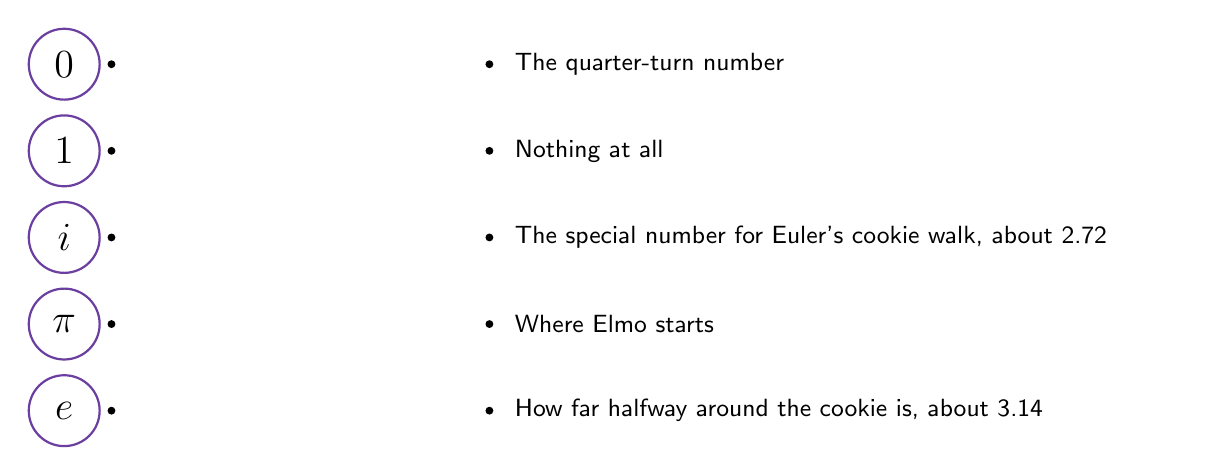
\begin{tikzpicture}
  \foreach \y/\n in {0/$0$, -1.1/$1$, -2.2/$i$, -3.3/$\pi$, -4.4/$e$}
    \node[draw=itc, line width=0.8pt, circle, minimum size=0.9cm, font=\Large] at (0,\y) {\n};
  \foreach \y in {0,-1.1,-2.2,-3.3,-4.4} {
    \fill (0.6,\y) circle (0.05);
    \fill (5.4,\y) circle (0.05);
  }
  \foreach \y/\t in {0/{The quarter-turn number},
                     -1.1/{Nothing at all},
                     -2.2/{The special number for Euler's cookie walk, about 2.72},
                     -3.3/{Where Elmo starts},
                     -4.4/{How far halfway around the cookie is, about 3.14}}
    \node[right, text width=8.5cm, font=\small] at (5.6,\y) {\t};
\end{tikzpicture}
\end{center}

\begin{tcolorbox}[enhanced, colback=white, colframe=robo, boxrule=1pt, arc=3mm,
  height=5.5cm, title={\textbf{Draw it!}}, colbacktitle=robo, coltitle=white]
Draw Elmo walking halfway around Cookie Monster's giant cookie, from $1$ to $-1$. Write
$e^{i\pi} = -1$ next to your picture.
\end{tcolorbox}

{\small\color{gray}\textbf{For teachers:} multiplying by $i$ rotates the complex plane by
$90^\circ$ counterclockwise, which is why $i^2 = -1$ reads as two quarter turns making a half
turn. Euler's formula $e^{i\theta} = \cos\theta + i\sin\theta$ places $e^{i\theta}$ on the unit
circle at arc length $\theta$ from $1$ (counterclockwise), so $\theta = \pi$ lands on $-1$.
The ``cookie 2 steps wide'' is the unit circle (radius 1), whose circumference is $2\pi$.
Why $e$ in particular is the base that turns ``growth'' into ``rotation'' is a calculus fact
($\tfrac{d}{d\theta}e^{i\theta} = i\,e^{i\theta}$: the velocity is always a quarter turn from
the position) and is beyond this worksheet. Sesame Street characters appear by name only, for
classroom use; this worksheet is not affiliated with or endorsed by Sesame Workshop.}

% ================= Answer key =================
\newpage
\section{Answer key}

\begin{center}
\rowcolors{2}{white}{softyellow}
\begin{tabularx}{\linewidth}{|>{\centering\arraybackslash}p{2.8cm}|X|}
\hline
\rowcolor{robodark}
\textbf{\color{white}Question} & \textbf{\color{white}Answer} \\ \hline
1 & $-4$ \\ \hline
2 & $2$; facing forward again (the way the numbers grow) \\ \hline
3 & $1 \times 1 = 1$, no; $(-1)\times(-1) = 1$, no \\ \hline
Turning table &
  \begin{tabular}[t]{@{}lll@{}}
    2 turns: & $-1$, & left \\
    3 turns: & $-i$, & down \\
    4 turns: & $1$, & right
  \end{tabular} \\ \hline
4 & 4 quarter turns \\ \hline
5 & $1$ (8 is two groups of 4) \\ \hline
6 & B is $-2 + 3i$; C is $3 + (-2)i$, which is also written $3 - 2i$ \\ \hline
7 & A cookie one step right, three steps up \\ \hline
8 & A little more than 3 (about 3.14 if measured carefully) \\ \hline
Circle boxes & Quarter way: $i$; halfway: $-1$; three-quarters: $-i$ \\ \hline
9 & $-1$ \\ \hline
10 & $0$; so $e^{i\pi} + 1 = 0$ \\ \hline
11 & $0$: nothing at all; $1$: where Elmo starts; $i$: the quarter-turn number;
     $\pi$: halfway around, about 3.14; $e$: Euler's special number, about 2.72 \\ \hline
\end{tabularx}
\end{center}

\end{document}
